%        File: arfc-beamer.tex
%     Created: Sun May 5 10:00 PM 2013 C


%\documentclass[11pt,handout]{beamer}
\documentclass[9pt]{beamer}
\usetheme[white]{Illinois}
%\title[short title]{long title}
\title[DDCA]{Demand Driven Cycamore Archetypes}
%\subtitle[short subtitle]{long subtitle}
\subtitle[DE-10512]{FY16 NEUP Award Summary}
%\author[short name]{long name}
\author[ARFC]{\textbf{Kathryn Huff}\\
Gwendolyn Chee, Roberto Fairhurst, Robert Flanagan, 
Jin Whan Bae, Anthony Scopatz, Travis Knight}
%\date[short date]{long date}
\date[09.17.2019]{September 17, 2019}
%\institution[short name]{long name}
\institute[UIUC]{University of Illinois at Urbana-Champaign}

%\usepackage{bbding}
\usepackage{amsfonts}
\usepackage{amsmath}
\usepackage{xspace}
\usepackage{graphicx}
\usepackage{subfigure}
\usepackage{booktabs} % nice rules for tables
\usepackage{microtype} % if using PDF
\usepackage{bigints}
\usepackage{minted}



\newcommand{\Cyclus}{\textsc{Cyclus}\xspace}%
\newcommand{\Cycamore}{\textsc{Cycamore}\xspace}%
\newcommand{\deploy}{\texttt{d3ploy}\xspace}%
\newcommand{\units}[1] {\:\text{#1}}%
\newcommand{\SN}{S$_N$}%{S$_\text{N}$}%{$S_N$}%
\DeclareMathOperator{\erf}{erf}
%I need some complimentary error funcitons...
\DeclareMathOperator{\erfc}{erfc}
%page numbers
\setbeamertemplate{footline}[page number]
\setbeamertemplate{caption}[numbered]
%Those icons in the references are terrible looking
\setbeamertemplate{bibliography item}[text]

%Gwen Tikz additions
\usepackage{tikz}
\usetikzlibrary{positioning, arrows, decorations, shapes}

\usetikzlibrary{shapes.geometric,arrows}
\tikzstyle{process} = [rectangle, rounded corners, minimum width=3cm, minimum height=1cm,text centered, draw=black, fill=blue!30]
\tikzstyle{object} = [ellipse, rounded corners, minimum width=3cm, minimum height=1cm,text centered, draw=black, fill=green!30]
\tikzstyle{arrow} = [thick,->,>=stealth]

\definecolor{illiniblue}{HTML}{B1C6E2}
\definecolor{illiniorange}{HTML}{f8c2a2}
\usetikzlibrary{shapes.geometric, arrows}
\tikzstyle{oblock} = [rectangle, draw, fill=illiniorange,
text width=15em, text centered, rounded corners, minimum height=4em]
\tikzstyle{bblock} = [rectangle, draw, fill=illiniblue,
text width=15em, text centered, rounded corners, minimum height=4em]
\tikzstyle{arrow} = [thick,->,>=stealth]

\usepackage{tabularx}
\newcolumntype{b}{>{\hsize=1.0\hsize}X}
\newcolumntype{s}{>{\hsize=.5\hsize}X}
\newcolumntype{m}{>{\hsize=.75\hsize}X}
\newcolumntype{x}{>{\hsize=.25\hsize}X}
\newcolumntype{L}{>{\raggedright\arraybackslash}X}
\newcolumntype{R}{>{\raggedleft\arraybackslash}X}
\def\arraystretch{1}
%%%% Acronym support
\usepackage{multirow}
\usepackage{graphicx,subfigure}


%%%% Acronym support

\usepackage[acronym,toc]{glossaries}
\include{acros}

\makeglossaries

%try to get rid of header on title page\dots
\makeatletter
    \newenvironment{withoutheadline}{
        \setbeamertemplate{headline}[default]
        \def\beamer@entrycode{\vspace*{-\headheight}}
    }{}
\makeatother

\makeatother
\setbeamertemplate{footline}
{
  \leavevmode%
  \hbox{%
    \rightline{\insertframenumber{} / \inserttotalframenumber\hspace*{1ex}}
  }%
  \vskip0pt%
}
\makeatletter

\begin{document}
%%%%%%%%%%%%%%%%%%%%%%%%%%%%%%%%%%%%%%%%%%%%%%%%%%%%%%%%%%%%%
%% From uw-beamer Here's a handy bit of code to place at 
%% the beginning of your presentation (after \begin{document}):
\newcommand*{\alphabet}{ABCDEFGHIJKLMNOPQRSTUVWXYZabcdefghijklmnopqrstuvwxyz}
\newlength{\highlightheight}
\newlength{\highlightdepth}
\newlength{\highlightmargin}
\setlength{\highlightmargin}{2pt}
\settoheight{\highlightheight}{\alphabet}
\settodepth{\highlightdepth}{\alphabet}
\addtolength{\highlightheight}{\highlightmargin}
\addtolength{\highlightdepth}{\highlightmargin}
\addtolength{\highlightheight}{\highlightdepth}
\newcommand*{\Highlight}{\rlap{\textcolor{HighlightBackground}{\rule[-\highlightdepth]{\linewidth}{\highlightheight}}}}
%%%%%%%%%%%%%%%%%%%%%%%%%%%%%%%%%%%%%%%%%%%%%%%%%%%%%%%%%%%%%
%%--------------------------------%%
\begin{withoutheadline}
\frame{
  \titlepage
}
\end{withoutheadline}

%%--------------------------------%%
\AtBeginSection[]{
\begin{frame}
  \frametitle{Outline}
  \tableofcontents[currentsection]
\end{frame}
}

\section{Overview}
\subsection{Motivation}
\begin{frame}
  \frametitle{Why Automate Fuel Cycle Deployment?}
  % a comment
  \begin{itemize}
      \item[$\bullet$] Automating deployments to meet power demands can be difficult for complicated
                       transition scenarios. 
      \item[$\bullet$] The deployment of reactors to create a balanced closed fuel cycle can be a 
                       complicated process. Ensuring that there is enough fast reactor fuel for
                       their operation requires the appropriate support fleet of light water reactors.
      \item[$\bullet$] Additionally, requiring users figure out the correct number of support
                       structures for the reactors fleets is a tedious job for humans.
   \end{itemize}        
\end{frame}

% key challenge
% funded milestones
\subsection{Objectives}
\input{objectives}

\section{Accomplishments}
\subsection{GIS Capability}
\input{gis}
\begin{frame}
        \frametitle{Synergistic Spent Nuclear Fuel Dynamics Within the European 
        Union}
\begin{itemize}
       \item Collaborative spent fuel management is materially feasible among nuclear
               nations in the  European Union.
       \item Collaborative EU spent fuel management could expedite a fast reactor
               technology transition in France.
       \item By using spent fuel from other EU nations, France can avoid
               building new light water reactors to support a transition to
               fast reactors.
\end{itemize}
\end{frame}


\begin{frame}
	\frametitle{Deployment Timeline for French Transition}
	110 SFRs (66 GWe) are deployed by 2076.
	\begin{figure}[htbp!]
	\begin{minipage}[b]{.45\linewidth}
        \begin{center}
                \includegraphics[width=\textwidth]{./images/french-transition/power_plot.png}
        \end{center}
        \caption{French Transition into an SFR Fleet}
        \label{fig:sfr_num}
	\end{minipage}
	\hspace{.5cm}
	\begin{minipage}[b]{.45\linewidth}
		\centering
		\includegraphics[width=\textwidth]{./images/french-transition/sfr_deploy.png}
		\caption{Deployment of French SFRs and total installed capacity}
		\label{fig:dep}
	\end{minipage}
\end{figure}
\end{frame}



\begin{frame}
\begin{figure}[htbp!]
    \begin{center}
        \includegraphics[width=\textwidth]{./images/onesim.png}
    \end{center}
    \caption{The simulated nuclear power deployment scheme relies on used
        nuclear fuel collaboration among nations.
        The historical operation of EU reactors is followed by the French transition to SFRs.  The steep transition from 2040 to 2060 reflects the scheduled decommissioning of reactors built in the 1975-2000 era of aggressive nuclear growth in France.}
    \label{fig:tot_dep}
\end{figure}
\end{frame}


\subsection{\deploy} 
\begin{frame}
    \frametitle{\deploy Objectives}
    \textbf{\deploy's Main Objective}
    \vspace{0.3em}
    \\
    Minimize the number of time steps of undersupply or under capacity 
    of power.
    \vspace{1em}
    \\
    \textbf{\deploy's Sub-Objectives}
    \begin{itemize}
        \item Minimize the number of time steps of undersupply or under capacity 
        of any commodity.
        \item Minimize excessive oversupply of all commodities  
    \end{itemize} 
\end{frame}

\begin{frame}
    \frametitle{\deploy Input Parameters}
    \begin{table}[]
        \centering
        \caption{\deploy's required and optional input parameters with examples.}
		\label{tab:inputs}
            \footnotesize
			\begin{tabularx}{\textwidth}{l|LL}
			\hline
				& \textbf{Input Parameter}                                                           & \textbf{Examples}                                                                                                          \\ \hline
				\multirow{5}{*}{\textbf{Required}} & Demand driving commodity                                                           & Power, Fuel, Plutonium, etc.                                                                                                                      \\ 
														  & Demand equation                                                                    & P(t) = 10000, sin(t), 10000*t                                                                                                                 \\ \cline{2-3} 
														  & Facilities it controls                                                             & Fuel Fab, LWR reactor, SFR reactor, Waste repository, etc.                                                                                                      \\ \cline{2-3} 
														  & Capacities of the facilities                                                       & 3000 kg, 1000 MW, 50000 kg                                                                                                     \\ \cline{2-3} 
														  & Prediction method                                                                  & \begin{tabular}[c]{@{}l@{}}Power: fast fourier transform\\ Fuel: moving average\\ Spent fuel: moving average\end{tabular} \\ \cline{2-3} 
														  & Deployment driven by & Installed Capacity/Supply                                                                                                                    \\ \hline
				\multirow{4}{*}{\textbf{Optional}} & Supply/Capacity Buffer type                                                                        & Absolute                                                                                                                  \\ \cline{2-3} 
														  & Supply/Capacity Buffer size                                                                        & \begin{tabular}[c]{@{}l@{}}Power: 3000 MW\\ Fuel: 0 kg \\ Spent fuel: 0 kg\end{tabular}                                   \\ \cline{2-3} 
														  & Facility preferences                                                               & \begin{tabular}[c]{@{}l@{}}LWR reactor = 100-t\\ SFR reactor = t-100 \end{tabular}          \\ \cline{2-3} 
														  & Facility constraint                                                              & SFR reactor constraint = 5000kg of Pu            \\ \hline	
						\end{tabularx}
    \end{table}
\end{frame}

\begin{frame}
    \frametitle{\deploy logic flow}
    \begin{columns}
        \column[t]{8cm}
    \begin{figure}[]
        \centering
        \resizebox{0.8\textwidth} {0.5\height}{
        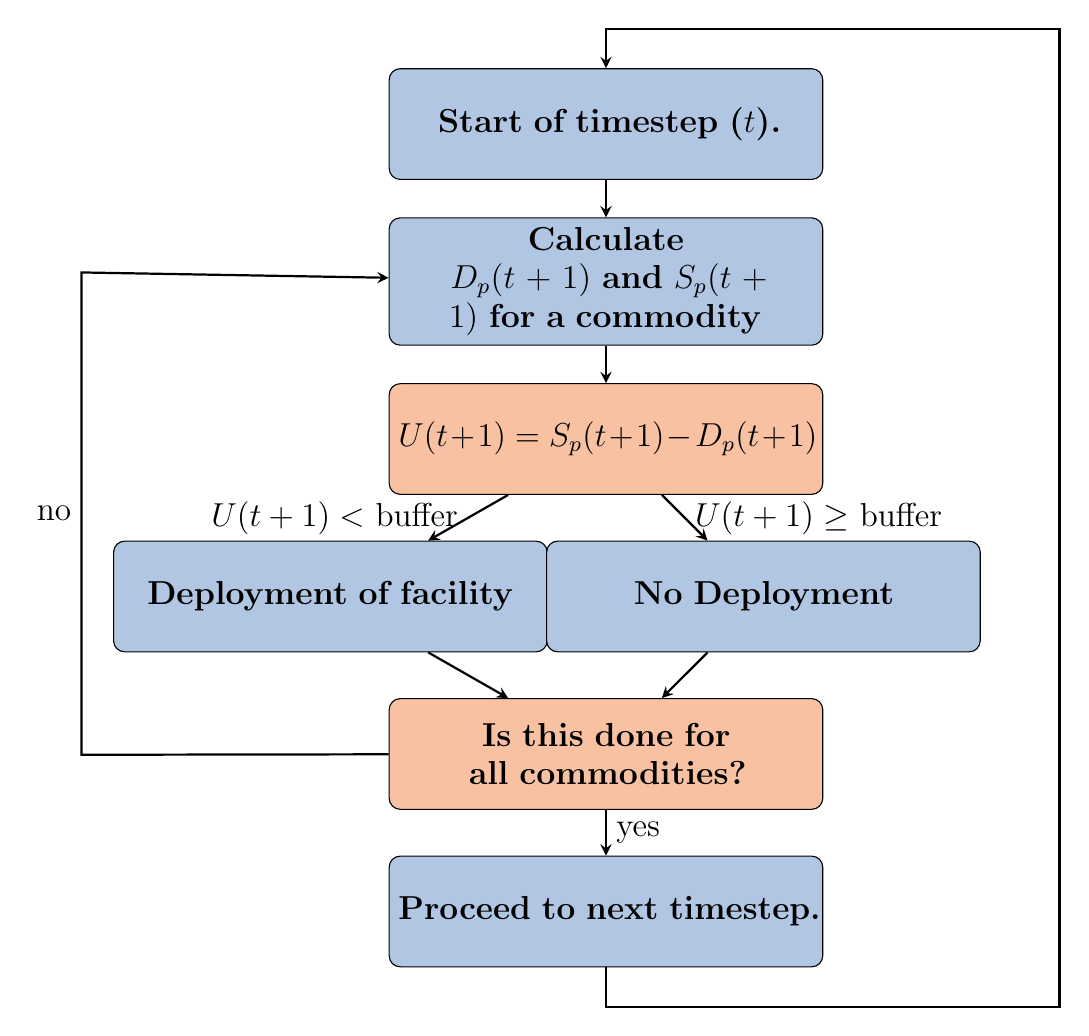
\begin{tikzpicture}[node distance=2cm]
        \tikzstyle{every node}=[font=\large]
        \node (Start) [bblock] {\textbf{Start of timestep ($t$).}};
        \node (Predict) [bblock, below of=Start] {\textbf{Calculate \\ $D_p(t+1)$ and $S_p(t+1)$ for a commodity}};
        \node (IsThere) [oblock, below of=Predict]{\textbf{$U(t+1) = S_p(t+1)-D_p(t+1)$}};
        \node (Deploy) [bblock, below of=IsThere, xshift = -3.5cm]{\textbf{Deployment of facility}};
        \node (NoDeploy) [bblock, right of=Deploy, xshift = 3.5cm]{\textbf{No Deployment} };
        \node (All) [oblock, below of=Deploy, xshift = 3.5cm] {\textbf{Is this done for all commodities?}};
        \node (End) [bblock, below of=All] {\textbf{Proceed to next timestep.}};
        
        \draw [arrow] (Start) -- (Predict); 
        \draw [arrow] (Predict) -- (IsThere);
        \draw [arrow] (IsThere) -- node[anchor=east] {$U(t+1) <$ buffer} (Deploy);
        \draw [arrow] (IsThere) -- node[anchor=west] {$U(t+1) \geq$ buffer} (NoDeploy);
        \draw [arrow] (Deploy) -- (All);
        \draw [arrow] (NoDeploy) -- (All);
        \draw [arrow] (All) -- node[anchor=west] {yes} (End);
        \draw [arrow] (All) -- ([shift={(-3.9cm,0.7cm)}]All.south west)-- node[anchor=east] {no} ([shift={(-3.9cm,-0.7cm)}]Predict.north west)--(Predict);
        \draw [arrow] (End) |-([shift={(3cm,-0.5cm)}]End.south east)-- ([shift={(3cm,0.5cm)}]Start.north east)-|(Start);
        \end{tikzpicture}
        }
        \caption{\deploy logic flow at every timestep in \Cyclus \cite{chee_demonstration_2019}.}
        \label{fig:flow}
    \end{figure}
    \column[t]{5cm}
    \vspace{2cm}
    \\
    $D_p : Predicted Demand$ \\
    $S_p : Predicted Supply$ \\
    $U = S_p-D_p$
\end{columns}
\end{frame}

\begin{frame}
    \frametitle{\deploy Prediction Methods}
    Non-Optimizing Methods 
    \begin{itemize}
        \item Moving Average (\texttt{ma})
        \item Autoregressive Moving Average (\texttt{arma})
        \item Autoregressive Heteroskedasticity (\texttt{arch})
    \end{itemize}
    Deterministic-Optimizing Methods 
    \begin{itemize}
        \item Fast Fourier Transform (\texttt{fft})
        \item Polynomial Fit (\texttt{poly})
        \item Exponential Smoothing
        \item Triple Exponential Smoothing (\texttt{holt-winters})
    \end{itemize}
    Stochastic-Optimizing Methods 
    \begin{itemize}
        \item Auto-Regressive Integrated Moving Averages (\texttt{ARIMA})
    \end{itemize}
\end{frame}
\begin{frame}
    \frametitle{Breakdown of Results}
    4 transition scenarios sought to minimize undersupply and under capacity of 
        all commodities.
    \begin{enumerate}
            \item EG01-23 ($P(t) = P_0$)
        \item EG01-24 ($P(t) = P_0 + rt$)
        \item EG01-29 ($P(t) = P_0)$
        \item EG01-30 ($P(t) = P_0 + rt$)
    \end{enumerate}

This is achieved by:
\begin{enumerate}
    \item Comparison of prediction methods for each of 4 scenarios is conducted 
    to determine the best method. 
    \item Sensitivity analysis of power supply buffer is conducted to determine 
    best buffer size. 
    \item Using best prediction method, look ahead rate, buffer size, demonstrate \deploy 
    deploying reactor and supporting facilities to meet power demand 
    for 4 scenarios. 
\end{enumerate}

\end{frame}


\begin{frame}
        \frametitle{EG01 - EG23}

\begin{figure}[H]
	\centering
	\includegraphics[width=\textwidth]{images/23flow.pdf}
	\hfill
	\caption{EG01-EG23 fuel cycle as modeled in \cyclus.}
	\label{fig:23flow}
\end{figure}
\end{frame}





\begin{frame}
        \frametitle{EG01 - EG23}

\begin{figure}[H]
	\centering
	\includegraphics[width=\textwidth]{images/30flow.pdf}
	\hfill
	\caption{EG01-EG30.}
	\label{fig:30flow}
\end{figure}


\subsection{Comparison of Prediction Methods}
\begin{frame}
    \frametitle{Comparison of Prediction Methods}
\textbf{EG01-23 Constant Power Demand Transition Scenario}

\begin{figure}[htbp!]
    \begin{center}
      \includegraphics[width=\textwidth]{../paper/figures/eg23-undersupply.png}
    \end{center}
          \caption{Time dependent undersupply of commodities for different
          prediction methods for the EG01-23 Transition Scenario with Constant Power Demand. The
          size of each cross is based on the size of the undersupply.
          Fewer crosses on plot indicates the method is more successful at preventing undersupply 
          of each commodity}
  \end{figure}
\end{frame}

\begin{frame}
    \frametitle{Comparison of Prediction Methods}
    \textbf{EG01-23 Constant Power Demand Transition Scenario}
\begin{figure}[htbp!]
    \begin{center}
      \includegraphics[width=\textwidth]{../paper/figures/eg23-undersupply.png}
    \end{center}
          \caption{Time dependent undersupply of commodities for different
          prediction methods for the EG01-23 Transition Scenario with Constant Power Demand. The
          size of each cross is based on the size of the undersupply.
          Fewer crosses on plot indicates the method is more successful at preventing under capacity 
          of each commodity}
  \end{figure}
\end{frame}

\begin{frame}
    \frametitle{Comparison of Prediction Methods}
\textbf{EG01-24 Constant Power Demand Transition Scenario}
\begin{figure}[htbp!]
    \begin{center}
      \includegraphics[width=\textwidth]{../paper/figures/eg24-undersupply.png}
    \end{center}
          \caption{Time dependent undersupply of commodities for different
          prediction methods for the EG01-24 Transition Scenario with Linearly Increasing Power Demand.The
          size of each cross is based on the size of the undersupply.
          Fewer crosses on plot indicates the method is more successful at preventing undersupply 
          of each commodity}
  \end{figure}
\end{frame}

\begin{frame}
    \frametitle{Comparison of Prediction Methods}
    \textbf{EG01-24 Constant Power Demand Transition Scenario}
\begin{figure}[htbp!]
    \begin{center}
      \includegraphics[width=\textwidth]{../paper/figures/eg24-undersupply.png}
    \end{center}
          \caption{Time dependent undersupply of commodities for different
          prediction methods for the EG01-24 Transition Scenario with Linearly Increasing Power Demand. The
          size of each cross is based on the size of the under capacity.
          Fewer crosses on plot indicates the method is more successful at preventing under capacity
          of each commodity}
  \end{figure}
\end{frame}

\begin{frame}
  \frametitle{Comparison of Prediction Methods}
  \textbf{Main Takeaway}
  \\
  The best performing prediction method for each transition scenario is: 
  \begin{enumerate}
    \item EG01-23 Constant Power Demand: \texttt{poly}
    \item EG01-24 Linearly Increasing Power Demand: \texttt{fft}
    \item EG01-29 Constant Power Demand: \texttt{poly}
    \item EG01-30 Linearly Increasing Power Demand: \texttt{fft}
\end{enumerate}
\end{frame}
\begin{frame}
    \frametitle{Sensitivity Analysis of Power Buffer}
    \textbf{EG01-24}: Linearly Increasing Power Demand
    \begin{figure}[htbp!]
        \begin{center}
          \includegraphics[width=0.8\textwidth]{images/24-sens-buffer}
        \end{center}
              \caption{Sensitivity Analysis of Power buffer size on cumulative 
              undersupply of Power for EG01-EG24 transition scenarios 
              with linearly increasing power demand using the fft prediction method.}
      \end{figure}
\end{frame}

\begin{frame}
    \frametitle{Sensitivity Analysis of Power Buffer}
    \textbf{EG01-30}: Linearly Increasing Power Demand
    \begin{figure}[htbp!]
        \begin{center}
          \includegraphics[width=0.8\textwidth]{images/30-sens-buffer}
        \end{center}
              \caption{Sensitivity Analysis of Power buffer size on cumulative 
              undersupply of Power for EG01-EG30 transition scenarios 
              with linearly increasing power demand using the fft prediction method.}
      \end{figure}
\end{frame}

\begin{frame}
  \frametitle{Sensitivity Analysis of Power Buffer}
  \textbf{Main Takeaway}
  \\
  The best power supply buffer for each transition scenario is: 
  \begin{enumerate}
    \item EG01-23 Constant Power Demand: 0 MW
    \item EG01-24 Linearly Increasing Power Demand: 6000 MW
    \item EG01-29 Constant Power Demand: 0 MW
    \item EG01-30 Linearly Increasing Power Demand: 8000 MW 
\end{enumerate}
\end{frame}

\begin{frame}
    \frametitle{Best Performing Transition Scenarios}
    \textbf{Input Parameters of best performing transition scenarios}
    \begin{table}[]
        \resizebox{\textwidth}{!}{%
        \begin{tabular}{|l|l|c|l|l|l|}
        \hline
        \multirow{2}{*}{}                         & \multicolumn{1}{c|}{\multirow{2}{*}{\textbf{Input Parameter}}} & \multicolumn{4}{c|}{\textbf{Simulation Description}}                                                                                                                                                                                                                                                       \\ \cline{3-6} 
                                                  & \multicolumn{1}{c|}{}                                          & \multicolumn{1}{l|}{\textbf{EG01-23}}                                                                 & \textbf{EG01-24}                  & \textbf{EG01-29}                 &\textbf{EG01-30}                                                  \\ \hline
        \multirow{4}{*}{\textbf{Required}} & Demand driving commodity                                       & \multicolumn{4}{c|}{Power}                                                                                                                                                                                                                                                                                 \\ \cline{2-6} 
                                                  & Demand equation [MW]                                               & \multicolumn{1}{l|}{60000}                                                                                & $60000 + 250t/12$ & 60000                     &     $60000 + 250t/12$                                       \\ \cline{2-6} 
                                                  & Prediction method                                              & \texttt{poly}       & \texttt{fft}             & \texttt{poly}         &  \texttt{fft}    \\ \cline{2-6} 
                                                  & Deployment Driving Method                                      & \multicolumn{4}{c|}{Installed Capacity}                                                                                                                                                                                                                                                                    \\ \hline
        \multirow{2}{*}{\textbf{Optional}} & Buffer type                                                    & \multicolumn{4}{c|}{Absolute}                                                                                                                                                                                                                                                               \\ \cline{2-6} 
                                                  & Power Buffer size [MW]                                                   & 0 & 6000 & 0 & 8000 \\ \hline
        \end{tabular}%
        }
        \caption{\deploy's input parameters for EG01-EG23, EG01-EG24, EG01-EG29, and 
        EG01-EG30 transition scenarios
        that minimizes undersupply of power and minimizes 
        the undersupply and under capacity of the other facilities. }
        \label{tab:bestinputs}
        \end{table}
\end{frame}

\begin{frame}
    \frametitle{Best Performing Transition Scenarios}
    \textbf{EG01-23: Constant Power Demand}
    \begin{figure}[htbp!]
        \begin{center}
          \includegraphics[width=\textwidth]{images/eg23-stack_reactor.png}
        \end{center}
              \caption{Time dependent deployment of reactor facilities in 
              the EG01-23 constant power demand transition scenario. 
              \deploy automatically deploys reactor facilities 
              to set up a supply chain to meet constant power demand of $60000$ MW
              during a transition from \glspl{LWR} to \glspl{SFR}}.
      \end{figure}
\end{frame}

\begin{frame}
    \frametitle{Best Performing Transition Scenarios}
    \textbf{EG01-23: Constant Power Demand}
    \begin{figure}[htbp!]
        \begin{center}
          \includegraphics[width=\textwidth]{images/eg23-stack_support.png}
        \end{center}
              \caption{Time dependent deployment of supporting facilities in 
              the EG01-23 constant power demand transition scenario. 
              \deploy automatically deploys reactor facilities 
              to set up a supply chain to meet constant power demand of $60000$ MW
              during a transition from \glspl{LWR} to \glspl{SFR}}.
      \end{figure}
\end{frame}

\begin{frame}
    \frametitle{Best Performing Transition Scenarios}
    \textbf{EG01-30: Linearly Increasing Power Demand}
    \begin{figure}[htbp!]
        \begin{center}
          \includegraphics[width=\textwidth]{images/eg30-stack_reactor.png}
        \end{center}
              \caption{Time dependent deployment of reactor facilities in 
              the EG01-30 linearly increasing power demand transition scenario. 
              \deploy automatically deploys reactor facilities 
              to set up a supply chain to meet constant power demand of $60000+250t/12$ MW
              during a transition from \glspl{LWR} to \glspl{SFR}}.
      \end{figure}
\end{frame}

\begin{frame}
    \frametitle{Best Performing Transition Scenarios}
    \textbf{EG01-30: Linearly Increasing Power Demand}
    \begin{figure}[htbp!]
        \begin{center}
          \includegraphics[width=\textwidth]{images/eg30-stack_support.png}
        \end{center}
              \caption{Time dependent deployment of supporting facilities in 
              the EG01-30 linearly increasing power demand transition scenario. 
              \deploy automatically deploys reactor facilities 
              to set up a supply chain to meet constant power demand of $60000+250t/12$ MW
              during a transition from \glspl{LWR} to \glspl{SFR}}.
      \end{figure}
\end{frame}

\begin{frame}
    \frametitle{Best Performing Transition Scenarios}
    \textbf{Undersupply and under capacity of commodities for the best performing transition scenarios} 
    \begin{table}[]
        \centering
            \caption{Undersupply/capacity of commodities for the best performing EG01-EG23,24,29,30 transition scenarios.}
            \label{tab:all-power}
            \footnotesize
            \begin{tabularx}{\textwidth}{l|RRRR}
            \hline
            & \multicolumn{3}{|c}{\textbf{Undersupplied Time Steps}} \\ \hline
            \textbf{Transition Scenario} & EG01-EG23 & 
            EG01-EG24 & EG01-EG29 & 
            EG01-EG30 \\ 
            \textbf{Power Demand} &Constant&Linearly Increasing&Constant&Linearly Increasing \\
            \textbf{Prediction Method} &\texttt{poly}&\texttt{fft}&\texttt{poly}& \texttt{fft}\\
            \textbf{Power Supply Buffer [MW]} &0&6000&0&8000 \\ \hline
            \textbf{Commodities} \\ 
            Natural Uranium		    & 2 	& 3  &  1  & 1 \\ 
            \gls{LWR} Fuel     	    & 4 	& 6  &  1  & 2\\ 
            \gls{SFR} Fuel     	    &  0 	& 0  &  2  & 2\\ 
            \gls{MOX} \gls{LWR} Fuel &-&-&2&2 \\
            Power      				&  6 	& 7  &  4 &  5\\ 
            \gls{LWR} Spent Fuel	& 1 	& 1  & 1 & 1\\ 
            \gls{SFR} Spent Fuel     	    &  1 	& 1  &  1  & 1\\ 
            \gls{MOX} \gls{LWR} Spent Fuel &-&-&1&1 \\ \hline 
        \end{tabularx}
    \end{table}
    
\end{frame}

\section{Conclusion}
\subsection{Conclusion}
\begin{frame}
  \frametitle{Conclusion}
        These results demonstrate that by carefully selecting \deploy 
        parameters, we are able to \textbf{effectively automate deployment}
        of reactor and supporting facilities to set up 
        constant and linearly increasing power demand transition scenarios
        for EG01-23, EG01-24, EG01-29, and EG01-30 with minimal 
        power undersupply. 
        \vspace{1em}
        \\
        Not completely eliminating undersupply and under capacity of 
        commodities in the simulation is expected 
        since without time series data 
        at the beginning of the simulation, \deploy takes a few 
        time steps to collect time series data about power demand 
        to predict and start deploying reactor and supporting 
        fuel cycle facilities. 
        
\end{frame}

\subsection{Auxilliary Activities}
\input{acks}


%%--------------------------------%%
%%          Bibliography          %%
%%--------------------------------%%
\begin{frame}[allowframebreaks]
  \frametitle{References}
  \bibliographystyle{plain}
  {\footnotesize \bibliography{2019-09-17-anl.bib} }
\end{frame}

%%--------------------------------%%

% Examples 
% Robert: Some good examples of how to use beamer are in the example file.
% You can use this to guide the preparation of slides.


\end{document}

